\documentclass[11pt]{article}

\usepackage[letterpaper,top=2cm,bottom=2cm,left=3cm,right=3cm,marginparwidth=1.75cm]{geometry}
\usepackage{fancyhdr}
\usepackage{authblk}
\usepackage[numbers,sort&compress]{natbib}
\usepackage[colorlinks=true, allcolors=blue]{hyperref}
\usepackage{orcidlink}
\usepackage{amsmath}
\usepackage{graphicx}
\usepackage{subcaption}
\usepackage{xcolor}
\usepackage{lineno}
\usepackage{booktabs}
\usepackage{float} 
\usepackage{placeins}





\fancypagestyle{plain}{
  \fancyhf{}
  \renewcommand{\headrulewidth}{0pt}
  \renewcommand{\footrulewidth}{0pt}
}

\fancypagestyle{fancy}{
  \fancyhf{}
  \fancyfoot[C]{\thepage}
  \renewcommand{\headrulewidth}{0pt}
  \renewcommand{\footrulewidth}{0pt}
}

\pagestyle{fancy}


\title{A Comparative Study of Fine-Tuning BERT, BERT+LSTM, and BERT+RCNN for Vietnamese Sentiment Analysis}
\author{
Hoang Bao Viet, 
Nguyen Duc Gia Phuc, 
Nguyen Quang Tuan \\
The University of Danang, Vietnam - Korea University of Information and Communication Technology
}

\date{}

\begin{document}

\maketitle

\noindent
\hrule
\begin{abstract}
Sentiment analysis is a fundamental task in Natural Language Processing (NLP) that focuses on identifying and evaluating opinions expressed in text. This study explores the application of BERT-based models for sentiment analysis of Vietnamese user comments. We investigate and compare three fine-tuning approaches: the standard BERT model using the [CLS] token as input to a feed-forward neural network, a hybrid BERT+LSTM model, and a novel BERT+RCNN architecture that utilizes the full sequence of output vectors for classification. Experiments conducted on two Vietnamese sentiment datasets demonstrate that models leveraging BERT significantly outperform traditional deep learning baselines. Notably, our proposed BERT+RCNN approach consistently achieves the best performance, surpassing the standard BERT fine-tuning method in both accuracy and robustness.

\vskip 8pt
\noindent
{\it Keywords:} BERT, LSTM, RCNN, Vietnamese, Sentiment Analysis
\vskip 8pt
\noindent
\hrule
\vskip 8pt
\end{abstract}


\vspace{-20pt}
\section{Introduction}

In today's digital era, millions of user-generated comments are shared daily on social networks and e-commerce platforms. These comments provide valuable feedback for both consumers and service providers. However, due to the vast amount of data, it becomes impractical for humans to manually process and analyze such information. Therefore, there is a growing need for automated systems capable of identifying and evaluating users' opinions.

Sentiment analysis is a fundamental task in Natural Language Processing (NLP) that aims to determine the emotional tone behind textual content. A sentiment classification system can either predict fine-grained sentiment scores (e.g., from 1 to 5) or perform binary classification to detect whether the content expresses a \textit{positive} or \textit{negative} sentiment. In this study, we focus on the latter task.

In 2018, Devlin et al. \cite{BERTJacob} introduced BERT (Bidirectional Encoder Representations from Transformers), a pre-trained language representation model that has significantly advanced the state of the art across various NLP tasks. BERT captures the context of words by considering both left and right contexts simultaneously, making it particularly effective for understanding the sentiment expressed in text.

This paper investigates the application of BERT-based models to sentiment analysis in Vietnamese. We present and compare two approaches. The first is the original fine-tuning strategy introduced by Devlin et al., which uses the representation of the \texttt{[CLS]} token as input to a classification layer. The second approach, proposed in this paper, extends BERT by combining its contextual embeddings with additional neural architectures, including Long Short-Term Memory (LSTM) and Recurrent Convolutional Neural Network (RCNN) layers.

Our objective is to evaluate the effectiveness of these combined models and to demonstrate how different fine-tuning strategies can improve sentiment classification performance on Vietnamese datasets.

The remainder of this paper is organized as follows:  
\begin{itemize}
    \item Section~\ref{sec:related_work} reviews related work in sentiment analysis.
    \item Section~\ref{sec:background} introduces word embeddings, language models, and the BERT architecture.
    \item Section~\ref{sec:methodology} describes our two BERT-based fine-tuning methods.
    \item Section~\ref{sec:experiments} presents the experimental setup and results.
    \item Section~\ref{sec:conclusion} concludes the paper.
\end{itemize}

\section{Related Work}
\label{sec:related_work}

Sentiment analysis is a subtask of text classification in which the goal is to categorize textual data into sentiment classes, typically \textit{positive} or \textit{negative}. Early research in this field primarily relied on traditional machine learning techniques. One of the pioneering studies was conducted in 2002, where reviews were classified into positive and negative categories \cite{pang-etal-2002-thumbs}. This work utilized supervised learning models such as Support Vector Machines (SVM) \cite{article} and Naive Bayes classifiers \cite{dey2016sentiment} to perform sentiment classification. Another common approach employed sentiment lexicons, which use predefined dictionaries of emotionally charged words annotated with sentiment polarity and intensity \cite{taboada-etal-2011-lexicon}.

With the rise of deep learning, sentiment analysis has seen significant advancements through improved word and context representations. Kim \cite{zhang2015character} proposed the use of Convolutional Neural Networks (CNNs) for sentence classification, treating text as character-level input sequences. Mikolov et al.~\cite{mikolov2013distributed} introduced the Paragraph Vector model (also known as Doc2Vec), an unsupervised method for learning fixed-length representations of variable-length texts. Unlike traditional bag-of-words models, this approach learns document-level embeddings that capture semantic meaning \cite{mikolov2013distributedWord}.

In the context of Vietnamese language, Duyen et al. \cite{duyen} applied traditional classifiers such as Naive Bayes, Maximum Entropy, and SVM to review classification tasks on Agoda, a hotel booking platform. Their results indicated that the SVM model outperformed other approaches. On the deep learning front, Quan et al.~\cite{quan2019multi} proposed a hybrid architecture combining Long Short-Term Memory (LSTM) and CNN, named Multi-Channel LSTM-CNN, for Vietnamese sentiment analysis. This model outperformed standalone CNN and LSTM models. A similar approach was introduced in~\cite{vo2019deep}, where word vectors were first processed by a CNN layer, and the resulting feature maps were passed to an LSTM network for final sentiment classification. This pipeline demonstrated strong performance, especially for handling negative comments on social media platforms.

These studies demonstrate the evolution of sentiment analysis methods—from traditional machine learning and lexicon-based approaches to more powerful neural network architectures. However, few works have explored the integration of pre-trained language models like BERT for Vietnamese sentiment classification, which motivates our study.



\section{Background}
\label{sec:background}
\subsection{Word Embedding}

Word embedding refers to the process of representing words as dense vectors in a continuous vector space, typically of much lower dimensionality than the vocabulary size. This representation captures semantic and syntactic relationships between words. One of the earliest and most influential approaches is Word2Vec, proposed by Mikolov et al.~\cite{mikolov2013distributedWord}, which learns word representations by predicting surrounding words in a sentence using shallow neural networks.

Another widely used method is GloVe (Global Vectors for Word Representation), introduced by Pennington et al.~\cite{pennington-etal-2014-glove}, which combines the advantages of global matrix factorization and local context window methods to efficiently learn word vectors from large corpora.

More recently, contextual word embedding methods have emerged, with BERT (Bidirectional Encoder Representations from Transformers)~\cite{vaswani2017attention} being a prominent example. Unlike Word2Vec or GloVe, which produce a single vector per word, BERT generates dynamic word representations that depend on the context in which the word appears.

\subsection{Language Model}

A language model defines a probability distribution over sequences of words. Given a sequence $x_1, x_2, ..., x_n$, the language model estimates the joint probability:

\[
P(x_1, x_2, ..., x_n)
\]

where $n$ is the length of the sentence. Language models are essential for many NLP tasks such as machine translation, speech recognition, and text generation, as they can measure how likely a given sentence is within a language.

With the emergence of deep learning, large-scale pre-trained language models have become the foundation of modern NLP. These models are trained on massive text corpora and capture a wide range of linguistic knowledge. Once pre-trained, they can be fine-tuned on specific downstream tasks, leading to state-of-the-art performance in sentiment analysis, question answering, and more.

\subsection{BERT}

BERT is a deep bidirectional transformer-based language model introduced by Devlin et al.~\cite{BERTJacob}. It is built entirely on encoder layers from the original Transformer architecture~\cite{vaswani2017attention}, omitting the decoder blocks as they are not necessary for language understanding tasks.

Unlike previous models that process text in a left-to-right or right-to-left manner, BERT uses a masked language modeling (MLM) strategy to learn deep bidirectional representations. This allows BERT to better capture context and semantic nuances by simultaneously considering both left and right contexts of a word.

One of BERT’s key innovations is applying the self-attention mechanism bidirectionally during pre-training, significantly improving the quality of learned representations. As a result, BERT has set new benchmarks on multiple NLP tasks.

Two main configurations of BERT were introduced:
\begin{itemize}
    \item \textbf{BERT\textsubscript{BASE}}: 12 Transformer encoder layers, 12 self-attention heads, and 110 million parameters.
    \item \textbf{BERT\textsubscript{LARGE}}: 24 Transformer encoder layers, 16 self-attention heads, and 340 million parameters.
\end{itemize}



\section{Methodology}
\label{sec:methodology}
In this study, we explore two primary strategies for utilizing BERT in sentiment analysis of Vietnamese user comments: (1) feature extraction and (2) fine-tuning.

\subsection{Feature Extraction vs. Fine-Tuning}

\textbf{Feature Extraction:} In this approach, the BERT architecture is preserved as-is and used solely as a contextual feature generator. The output embeddings from BERT are extracted and then passed to a separate classification model. This strategy treats BERT as a frozen feature extractor without updating its internal weights.

\textbf{Fine-Tuning:} Fine-tuning involves extending the BERT model by adding task-specific layers (e.g., feed-forward layers for classification) and training the entire model, including BERT's internal parameters, on the target dataset. This method has been shown to yield significantly better performance compared to feature extraction, as demonstrated in the original BERT paper~\cite{BERTJacob} and in other benchmark evaluations such as the CoNLL-2003 Named Entity Recognition task~\cite{sang2003introduction}.

\subsection{BERT Pre-trained Model}

To fine-tune BERT effectively on Vietnamese data, a suitable pre-trained model is required. In our experiments, we adopt the \texttt{BERT-Base Multilingual Cased} model released by Google. This model is trained on 104 languages, including Vietnamese, and is case-sensitive (cased), preserving important features such as letter casing and diacritics — both critical in Vietnamese language processing.

\subsection{Fine-Tuning Approaches}

We experiment with two different fine-tuning strategies for sentiment classification:

\subsubsection{BERT with [CLS] Token Representation (BERT\textsubscript{base})}

Following the original setup by Devlin et al.~\cite{BERTJacob}, a special token \texttt{[CLS]} is added to the beginning of each input sequence. The final hidden state corresponding to this token is assumed to capture the entire sentence's meaning. This representation is passed through a feed-forward neural network for classification. The architecture of this model is illustrated in Figure~\ref{fig:bert_cls_architecture}.

\begin{figure}[h]
\centering
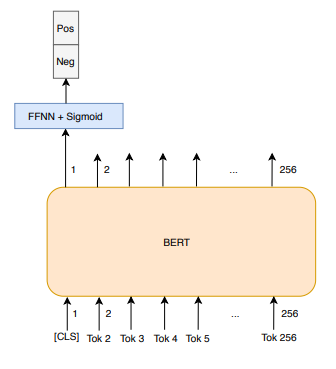
\includegraphics[width=0.45\textwidth]{img/BertBase.png}
\caption{Architecture BERT-base}
\label{fig:bert_cls_architecture}
\end{figure}
\FloatBarrier

\subsubsection{BERT with Full Token Representations}

In this method, we utilize the full sequence output of BERT, including the \texttt{[CLS]} token. The resulting output forms a matrix of shape $L \times h$, where $L$ is the maximum sequence length and $h$ is the hidden size of BERT embeddings (typically 768 in BERT\textsubscript{BASE}).

This output matrix is then used as input to more complex classification architectures, including:
\begin{itemize}
    \item \textbf{BERT+LSTM}: A bidirectional Long Short-Term Memory (LSTM) network captures sequential dependencies in the token embeddings.
    \item \textbf{BERT+RCNN}: A Recurrent Convolutional Neural Network combines the advantages of both LSTM and CNN to learn both global and local features.
\end{itemize}

The architecture for these models is depicted in Figure~\ref{fig:bert_rcnn_lstm_architecture}.

\begin{figure}[h]
\centering
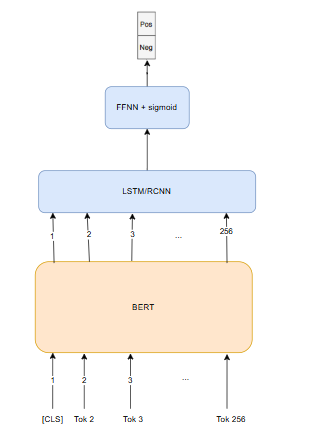
\includegraphics[width=0.45\textwidth]{img/BERTCombine.png}
\caption{Architecture BERT using all token}
\label{fig:bert_rcnn_lstm_architecture}
\end{figure}
\FloatBarrier

\section{Experiments}
\label{sec:experiments}
\subsection{Dataset}

To evaluate the effectiveness of different BERT-based architectures in Vietnamese sentiment analysis, we conducted experiments on a Vietnamese social media comment dataset. The dataset consists of user-generated reviews and comments collected from various online platforms, with each entry annotated as either \textit{positive} or \textit{negative} sentiment.

We preprocessed the dataset by removing special characters, normalizing Unicode, and tokenizing the text using a Vietnamese tokenizer. The dataset was then divided into a training set and a testing set using an 80/20 split. To ensure a balanced evaluation, both sets maintain an approximately equal distribution of positive and negative labels.

All models—BERT, BERT+LSTM, and BERT+RCNN—were trained and evaluated under the same conditions, using the pre-trained BERT-Base Multilingual Cased model as the backbone.

\subsection{Results and Discussion}

Table~\ref{tab:results} presents the performance comparison of the three models using Precision, Recall, and F1 Score as evaluation metrics.

The standard BERT model achieved the highest F1 Score of 90\%, indicating its strong capability to capture sentiment information from Vietnamese text. Although BERT+LSTM achieved comparable performance (F1 Score of 89\%), it did not significantly outperform the baseline BERT model. This suggests that the LSTM layer may introduce additional complexity without substantial gains in this binary classification task.

On the other hand, the BERT+RCNN model showed a noticeable decline in performance, with an F1 Score of 85\%. While the RCNN architecture is designed to capture both local and sequential features, its integration with BERT may have introduced redundancy or overfitting, especially on limited-size Vietnamese datasets.

Overall, the results demonstrate that fine-tuning BERT with minimal architectural changes provides the most robust and effective approach for Vietnamese sentiment classification. Additional layers such as LSTM or RCNN may not always lead to improved performance and should be used cautiously depending on dataset size and task complexity.



\begin{table}[h]
\centering
\caption{Performance Comparison on Sentiment Dataset}
\begin{tabular}{lccc}
\toprule
Model & Precision & Recall & F1 Score \\
\midrule
BERT & 88\% & 91\% & \textbf{90\%} \\
BERT + LSTM & 88\% & 90\% & 89\% \\
BERT + RCNN & 87\% & 83\% & 85\% \\
\bottomrule
\end{tabular}
\label{tab:results}
\end{table}


\section{Conclusion}
\label{sec:conclusion}
In this paper, we presented a comparative study on fine-tuning BERT for Vietnamese sentiment analysis. We explored three approaches: the standard BERT model utilizing the \texttt{[CLS]} token, a hybrid BERT+LSTM model, and a novel BERT+RCNN architecture that combines contextual embeddings with sequential and convolutional features.

Experimental results show that the standard BERT model achieves the highest F1 Score, demonstrating its effectiveness in capturing semantic information from Vietnamese text without additional architectural complexity. While the BERT+LSTM model offered comparable performance, the BERT+RCNN model underperformed, suggesting that adding more layers does not always improve results and may lead to overfitting on small or imbalanced datasets.

Our findings indicate that fine-tuning pre-trained multilingual BERT models is a powerful and efficient approach for Vietnamese sentiment classification. Future work may focus on exploring larger and more diverse datasets, experimenting with domain-specific pre-trained models, or applying cross-lingual transfer techniques to further improve performance in low-resource languages like Vietnamese.


\bibliographystyle{IEEEtran}
\bibliography{source.bib}

\end{document}
